\chapter{Anexo B: El Lenguaje Pure Data (Pd) y su Complejidad Estructural}
\label{anexo:pure_data}

Pure Data (Pd) es un entorno de programación visual de código abierto desarrollado originalmente por Miller Puckette en los años 90. Es ampliamente utilizado por músicos e investigadores para la creación interactiva de música por ordenador y obras multimedia. A diferencia de los lenguajes de programación tradicionales basados en texto, Pd permite a los usuarios desarrollar algoritmos conectando objetos gráficos en un \textit{lienzo} o, como Pure Data los denomina, \textit{patches}.

\section{Programación Visual en Pure Data}

En Pd, un programa se construye instanciando diferentes cajas u \textit{objetos} y conectándolos mediante \textit{cables}. Cada objeto realiza una función específica, como generar una onda matemática, sumar dos números o aplicar un filtro a una señal de audio.

El flujo de información viaja a través de las conexiones de arriba hacia abajo. Existen dos tipos principales de conexiones:
\begin{itemize}
    \item \textbf{Cables de control:} Transmiten mensajes y números discretos, ideales para enviar eventos, notas musicales o modificar parámetros en tiempo real.
    \item \textbf{Cables de señal (\textit{audio}):} Transmiten flujo continuo de audio a la frecuencia de muestreo del sistema (típicamente 44100 muestras por segundo). Los objetos que procesan estas señales se denotan con una tilde (\verb|~|) al final de su nombre (por ejemplo, \verb|osc~| o \verb|dac~|).
\end{itemize}

A continuación se muestra un ejemplo visual de un \textit{patch} básico en Pure Data:

\begin{figure}[H]
    \centering
    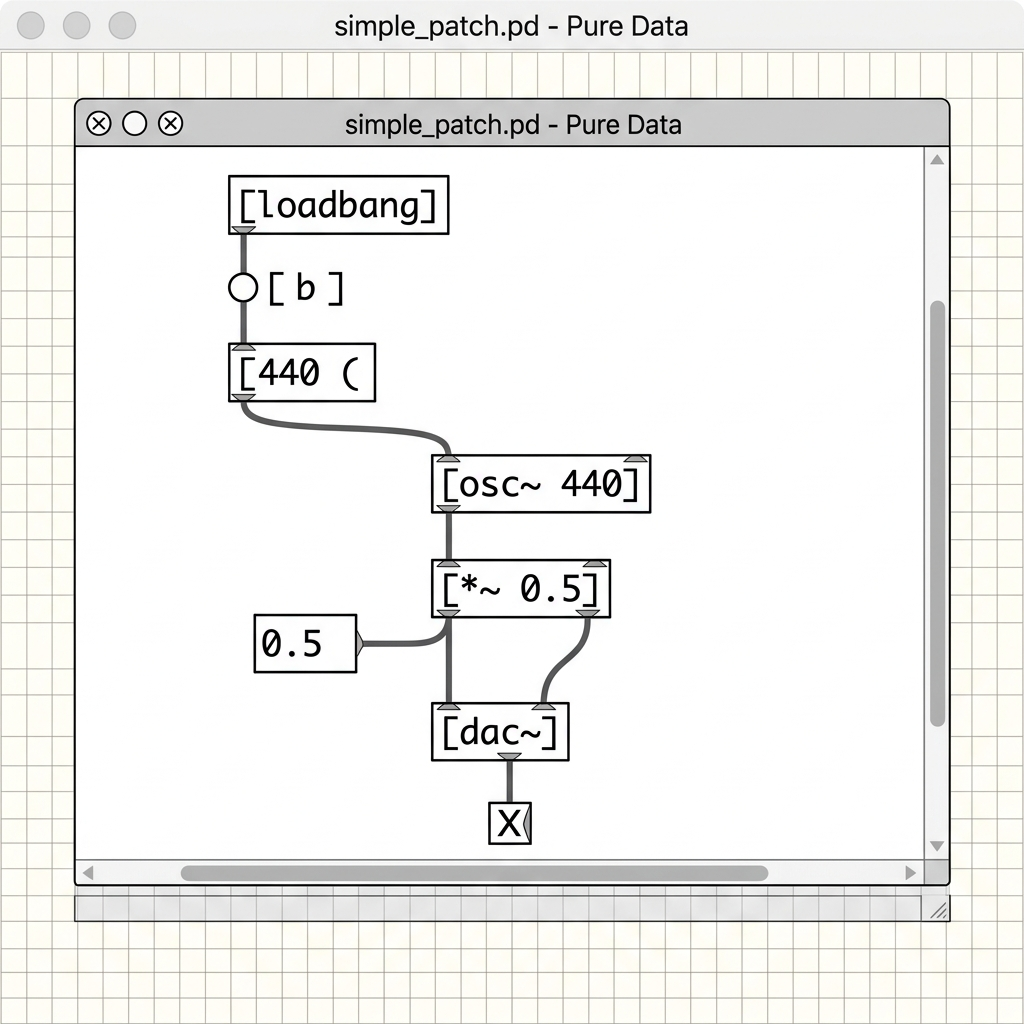
\includegraphics[width=0.7\textwidth]{imagenes/pure_data_patch.png}
    \caption{Interfaz visual de un \textit{patch} en Pure Data.}
    \label{fig:pure_data_patch}
\end{figure}
\subsection{Estructuración Modular: Subpatches y Abstracciones}

Al igual que en la ingeniería de software tradicional se utilizan funciones, métodos o clases para organizar y reutilizar el código, en Pure Data se emplea el concepto de \textit{patch} (el archivo principal o lienzo de trabajo) y sus encapsulaciones.

A medida que un sintetizador crece en complejidad, el lienzo visual puede volverse inmanejable. Para solucionar esto, Pd permite la creación de sub-módulos mediante dos mecanismos principales:
\begin{itemize}
    \item \textbf{Subpatches:} Se crean usando el objeto \verb|[pd nombre_del_subpatch]|. Al hacer doble clic sobre él, se abre una nueva ventana en blanco donde se puede seguir conectando objetos. Es útil para ocultar el desorden visual y agrupar lógica relacionada dentro del mismo archivo.
    \item \textbf{Abstracciones:} Consisten en guardar un \textit{patch} en un archivo \texttt{.pd} independiente y luego invocarlo desde otro \textit{patch} simplemente escribiendo su nombre en una caja de objeto. Esto permite la verdadera reutilización de código; por ejemplo, se puede diseñar un oscilador complejo y reutilizarlo múltiples veces instanciando su abstracción.
\end{itemize}

Desde la perspectiva de las herramientas de generación automática desarrolladas en este proyecto, este concepto de encapsulación es fundamental. Un sub-módulo en Pure Data equivale directamente al concepto arquitectónico de \textbf{\textit{Máquina}} definido en nuestros lenguajes DSL. Del mismo modo, esta misma equivalencia semántica se mapea a \textbf{clases} o \textbf{métodos} cuando el código objetivo es un lenguaje de texto estructurado como JavaScript u otros lenguajes soportados.

\section{Entorno Recomendado: Pd-l2ork (Purr Data)}

Aunque existe una versión original o \textit{vanilla} de Pure Data mantenida por Miller Puckette, para este proyecto y para el desarrollo moderno en general, se recomienda encarecidamente el uso de \textbf{Pd-l2ork} (también conocido en algunas de sus distribuciones como Purr Data). 

Esta bifurcación (\textit{fork}) del proyecto original ofrece una interfaz gráfica basada en tecnologías web mucho más amigable, mejoras significativas de usabilidad y un vasto conjunto de librerías y extensiones preinstaladas que facilitan la creación de sintetizadores sin necesidad de compilar dependencias de terceros.

\subsection{Instalación y Configuración Básica}
Pd-l2ork es multiplataforma y puede descargarse de forma gratuita desde su sitio web oficial  (\url{https://l2ork.bukvic.net/main/make-your-own-l2ork/software/}). La instalación sigue el proceso estándar de cualquier aplicación según el sistema operativo (Windows, macOS o Linux).



Un detalle crucial y un error extremadamente común entre los principiantes, es intentar hacer sonar un \textit{patch} sin haber activado el motor de audio del programa. Para que cualquier objeto relacionado con la síntesis de sonido (aquellos terminados en \verb|~|) genere salida acústica, es estrictamente necesario activar el procesamiento digital de señales.

\begin{figure}[H]
    \centering
    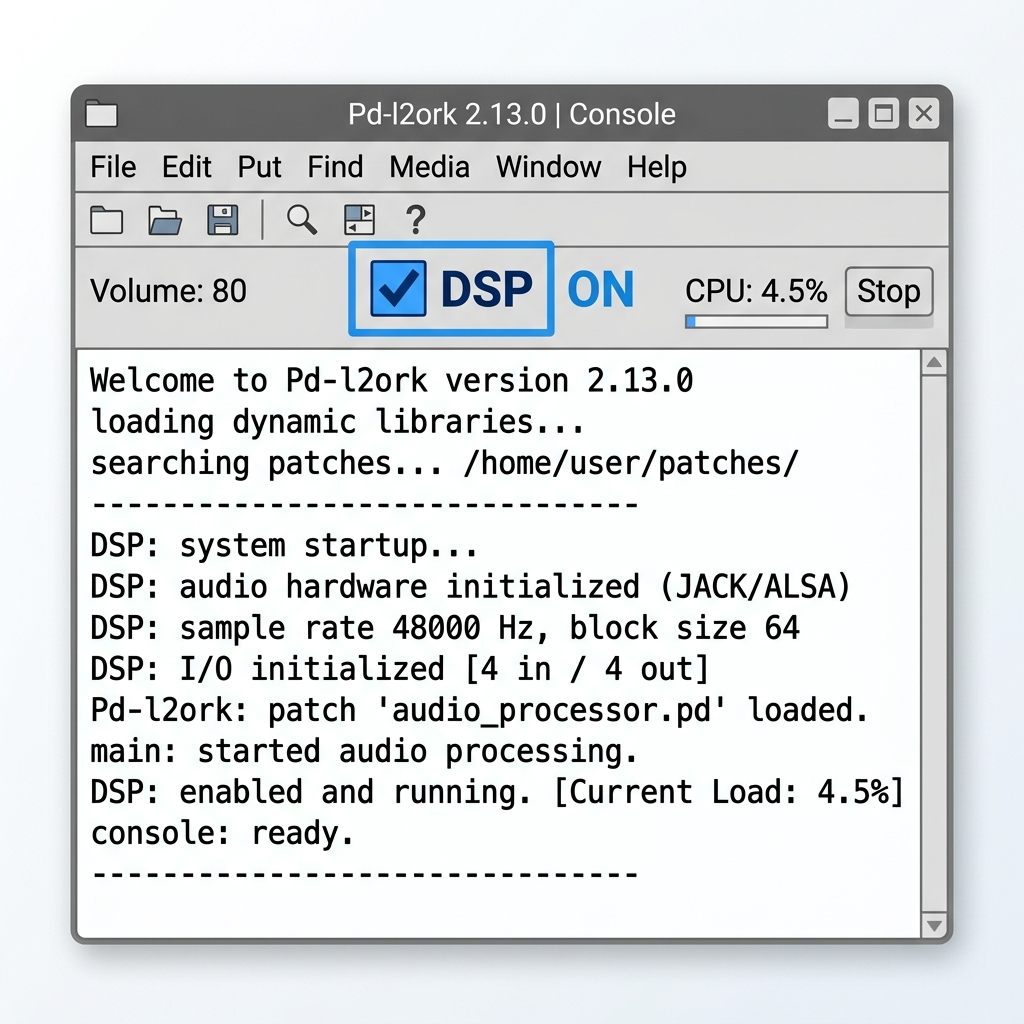
\includegraphics[width=0.6\textwidth]{imagenes/pdl2ork_dsp.png}
    \caption{Consola principal de Pd-l2ork destacando la casilla DSP.}
    \label{fig:pdl2ork_dsp}
\end{figure}

Para ello, basta con abrir la ventana principal (Consola) de Pd-l2ork y asegurarse de que la casilla etiquetada como \textbf{DSP} (\textit{Digital Signal Processing}) esté marcada, tal y como se observa en la Figura \ref{fig:pdl2ork_dsp}. Sin este paso, el \textit{patch} calculará datos de control, pero no emitirá ningún sonido.

\section{Estructura Interna del Archivo \texttt{.pd}}

A pesar de su interfaz visual e intuitiva, internamente Pure Data guarda estos \textit{patches} en un formato de texto plano (con extensión \texttt{.pd}). La sintaxis de este archivo es muy particular y está optimizada para ser leída rápidamente por el motor de Pd, no por un humano.

El siguiente es un ejemplo de cómo se representa internamente un \textit{patch} sencillo:

\begin{lstlisting}[language=bash, caption={Contenido en texto plano de un archivo \texttt{.pd}.}]
#N canvas 50 50 450 300 10;
#X obj 100 100 osc~ 440;
#X obj 100 150 *~ 0.5;
#X obj 100 200 dac~;
#X connect 0 0 1 0;
#X connect 1 0 2 0;
#X connect 1 0 2 1;
\end{lstlisting}

Como se observa, el formato define:
\begin{itemize}
    \item Definiciones del \textit{canvas} (coordenadas y tamaño de la ventana).
    \item Declaración de objetos (\verb|#X obj|) junto a sus coordenadas absolutas (X, Y) y sus parámetros de inicialización.
    \item Declaraciones de conexión (\verb|#X connect|), las cuales no hacen referencia a los identificadores o nombres de los objetos, sino a sus \textbf{índices de creación relativos} en el archivo, seguidos del índice del puerto de salida y el puerto de entrada respectivo.
\end{itemize}

\section{Desafíos para la Generación Automática}

La estructura de los archivos \texttt{.pd} presenta una extrema fragilidad. El hecho de que las conexiones dependan exclusivamente del índice posicional numérico de la línea en la que se declaró el objeto significa que cualquier reordenamiento en el archivo, o la inserción de un nuevo elemento sin recalcular minuciosamente todas las conexiones de índices, corrompe completamente el programa y sus relaciones.

Además, el formato \texttt{.pd} carece de una documentación oficial estandarizada de su gramática o de algoritmos claros para las coordenadas espaciales, las cuales son requeridas para que los objetos y cables no se dibujen superpuestos de forma caótica.

Esta inherente complejidad estructural, sumada a la falta de semántica explícita (basada en nombres o UUIDs), dificulta enormemente la generación automática directa de código para Pure Data mediante inteligencia artificial. Es precisamente esta barrera la que justifica y hace indispensable el uso de metodologías dirigidas por modelos (MDA) y DSL estructurados. Al contar con un modelo formal y abstracto, se puede aislar esta complejidad y delegar a un transpilador determinista la compleja y propensa a errores tarea de generar la sintaxis \texttt{.pd} válida.
